\documentclass[11pt,a4paper]{article}

% =============================================================================
% Backtest V2 Architecture Document
% =============================================================================

% Packages
\usepackage[utf8]{inputenc}
\usepackage[T1]{fontenc}
\usepackage{lmodern}
\usepackage[margin=1in]{geometry}
\usepackage{hyperref}
\usepackage{xcolor}
\usepackage{graphicx}
\usepackage{amsmath}
\usepackage{booktabs}
\usepackage{tabularx}
\usepackage{enumitem}
\usepackage{fancyhdr}
\usepackage{tocloft}
\usepackage{tikz}
\usetikzlibrary{shapes,arrows,positioning,fit,calc}

% Hyperref setup
\hypersetup{
    colorlinks=true,
    linkcolor=blue,
    filecolor=magenta,
    urlcolor=cyan,
}

% Styling helpers
\definecolor{boxblue}{RGB}{220,235,255}
\definecolor{boxgreen}{RGB}{224,245,228}
\definecolor{boxorange}{RGB}{255,238,220}
\definecolor{boxgray}{RGB}{245,245,245}
\definecolor{boxpurple}{RGB}{235,225,255}

% Header/Footer
\pagestyle{fancy}
\fancyhf{}
\rhead{BetterSys Architecture}
\lhead{Backtest V2}
\rfoot{Page \thepage}

% Title
\title{%
    \textbf{Backtest V2: Deterministic HFT Backtesting Architecture}\\
    \large High-Level System Design for Polymarket-Style CLOB Simulation
}
\author{System Documentation}
\date{January 2026}

\begin{document}

\maketitle
\tableofcontents
\newpage

% =============================================================================
\section{Executive Summary}
% =============================================================================

\textbf{Backtest V2} is a deterministic, event-driven backtesting framework designed to simulate high-frequency trading (HFT) strategies on Polymarket-style binary-outcome central limit order books (CLOBs). The system emphasizes three core properties:
\begin{enumerate}[leftmargin=*,itemsep=2pt]
    \item \textbf{Determinism:} identical inputs produce identical outputs across runs.
    \item \textbf{Microstructure realism:} FIFO matching, partial fills, order types, venue rules, and latency modeling.
    \item \textbf{Production-identical strategy surface:} strategies interact through a stable interface that can be backed by either a live gateway or a simulator.
\end{enumerate}

At a high level, a \texttt{BacktestOrchestrator} owns a monotonic \texttt{SimClock}, an \texttt{EventQueue} that enforces stable ordering, and an order adapter (\texttt{SimulatedOrderSender}) that routes strategy actions into a matching simulator (\texttt{MatchingEngine} + \texttt{LimitOrderBook}). Optional subsystems provide richer realism and analysis: order management (OMS), risk checks and Kelly sizing, portfolio accounting and settlement, comprehensive metrics, reproducibility validation, tracing, and performance tooling.

% =============================================================================
\section{Design Goals and Non-Goals}
% =============================================================================

\subsection{Primary Design Goals}
\begin{table}[h]
\centering
\small
\begin{tabularx}{\textwidth}{@{}lX@{}}
\toprule
\textbf{Goal} & \textbf{Interpretation in Backtest V2} \\
\midrule
Deterministic replay & No dependence on system time; deterministic event ordering; seeded RNG only; stable tie-break rules when timestamps match. \\
Realistic exchange behavior & FIFO queues at each price; tick discretization; maker/taker fees; post-only behavior; time-in-force; self-trade prevention; cancel acknowledgments. \\
Strategy portability & Strategy callbacks and order interface are consistent with a live execution surface; adapters swap without changing strategy logic. \\
Latency-aware simulation & End-to-end latency components are modelable (market data, decision time, send latency, venue latency, cancel latency, fill reporting), with optional tail behavior. \\
Auditability and debugging & Trace mode for event-by-event inspection; invariant checks; reproducibility fingerprints; replay test harness. \\
Scalability & Optional pooling and per-market isolation; benchmarking and profiling support; parallelizable processing model. \\
\bottomrule
\end{tabularx}
\caption{Primary design goals}
\end{table}

\subsection{Explicit Non-Goals (Current Scope)}
\begin{itemize}[leftmargin=*,itemsep=2pt]
    \item \textbf{Perfect venue emulation:} Backtest V2 targets realistic \emph{structure} (FIFO matching, rule surfaces, latency), not a complete reproduction of every exchange edge case.
    \item \textbf{Exchange-wide cross-instrument constraints:} Some subsystems model per-token books; full cross-token global order-id and global risk constraints may require additional orchestration.
    \item \textbf{Full on-chain settlement pipeline:} Settlement and outcome accounting are modeled abstractly; on-chain custody is outside the backtest engine.
\end{itemize}

% =============================================================================
\section{Core Abstractions and Type System}
% =============================================================================

Backtest V2 uses a small set of canonical primitives to keep the simulator composable.

\subsection{Time Model}
All simulation time is represented in nanoseconds (\texttt{Nanos}). A dedicated monotonic clock (\texttt{SimClock}) is the only time source.

\begin{table}[h]
\centering
\small
\begin{tabularx}{\textwidth}{@{}lX@{}}
\toprule
\textbf{Concept} & \textbf{Semantics} \\
\midrule
Simulation time (\texttt{Nanos}) & Monotonic, event-driven time used to timestamp all market and order events. \\
Event timestamp & The simulated ``exchange time'' at which an event becomes visible to the orchestrator and strategy. \\
Wall time & Used only to measure performance of the backtest run itself (e.g., elapsed milliseconds for throughput reporting). \\
\bottomrule
\end{tabularx}
\caption{Time model in Backtest V2}
\end{table}

\subsection{Market/Token Model}
Prediction markets are represented as binary-outcome instruments. Operationally, Backtest V2 treats each \emph{outcome token} as its own order book.

\begin{table}[h]
\centering
\small
\begin{tabularx}{\textwidth}{@{}lX@{}}
\toprule
\textbf{Identifier} & \textbf{Meaning} \\
\midrule
\texttt{token\_id} & Outcome-level token identifier (e.g., a Polymarket \emph{clobTokenId}); used to route book updates and orders to a specific book. \\
\texttt{market\_id} & Market-level identifier (e.g., event/condition). Portfolio accounting may track YES/NO outcomes under a market umbrella. \\
\texttt{Outcome} & Binary outcome (YES/NO) used for settlement and complement coupling in portfolio/risk subsystems. \\
\bottomrule
\end{tabularx}
\caption{Market and token identity (conceptual mapping)}
\end{table}

\subsection{Event Model}
All inputs and simulator outputs are expressed as canonical events. Each event carries an intrinsic \emph{priority class} used for deterministic ordering within the same timestamp.

\begin{figure}[h]
\centering
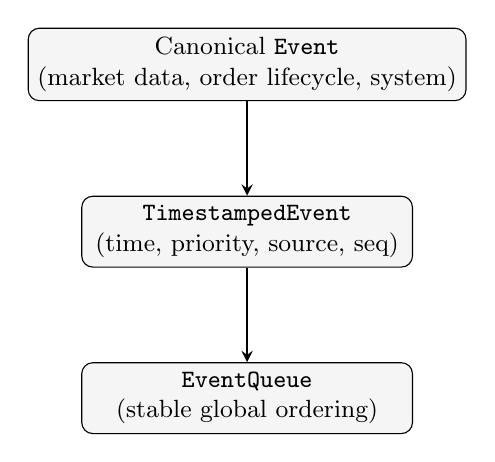
\begin{tikzpicture}[
    node distance=1.2cm,
    box/.style={rectangle, draw, rounded corners, align=center, minimum width=4.2cm, minimum height=0.9cm, font=\small, fill=boxgray},
    arrow/.style={->, >=stealth, thick}
]
    \node[box] (e) {Canonical \texttt{Event}\\(market data, order lifecycle, system)};
    \node[box, below=of e] (ts) {\texttt{TimestampedEvent}\\(time, priority, source, seq)};
    \node[box, below=of ts] (q) {\texttt{EventQueue}\\(stable global ordering)};

    \draw[arrow] (e) -- (ts);
    \draw[arrow] (ts) -- (q);
\end{tikzpicture}
\caption{Canonical event representation}
\end{figure}

\subsection{Stable Ordering Key}
Backtest V2 enforces deterministic ordering by sorting events lexicographically by:
\[
\textbf{key}(\text{event}) = (t,\; p,\; s,\; q)
\]
where:
\begin{itemize}[leftmargin=*,itemsep=2pt]
    \item $t$ = event timestamp in nanoseconds,
    \item $p$ = event priority class (system events before market data, before order events, before signals),
    \item $s$ = source stream (exchange, market data, signals, OMS/matching, timers, strategy),
    \item $q$ = per-source sequence number assigned on insertion (stable tie-break).
\end{itemize}

\begin{table}[h]
\centering
\small
\begin{tabular}{@{}ll@{}}
\toprule
\textbf{Ordering Field} & \textbf{Why it exists} \\
\midrule
Timestamp ($t$) & Preserves temporal causality. \\
Priority ($p$) & Ensures critical system transitions and market state are processed before dependent computations. \\
Source ($s$) & Stabilizes merges across heterogeneous streams when timestamps match. \\
Sequence ($q$) & Guarantees insertion stability when all other keys tie. \\
\bottomrule
\end{tabular}
\caption{Deterministic ordering rationale}
\end{table}

% =============================================================================
\section{High-Level Component Architecture}
% =============================================================================

\begin{figure}[h]
\centering
\begin{tikzpicture}[
    node distance=1.2cm,
    comp/.style={rectangle, draw, rounded corners, align=center, minimum width=3.6cm, minimum height=0.85cm, font=\small},
    core/.style={comp, fill=boxblue},
    sim/.style={comp, fill=boxgreen},
    opt/.style={comp, fill=boxorange},
    aux/.style={comp, fill=boxpurple},
    arrow/.style={->, >=stealth, thick},
    dashed/.style={->, >=stealth, thick, dashed}
]
    % Core orchestrator and queue
    \node[core] (orch) {BacktestOrchestrator\\(event loop + determinism)};
    \node[core, below=of orch] (queue) {EventQueue\\(time, priority, source, seq)};
    \node[core, left=2.2cm of queue] (clock) {SimClock\\(monotonic nanos)};

    % Inputs
    \node[sim, left=2.2cm of orch] (feed) {MarketDataFeed\\(historical replay)};
    \node[aux, above=of feed] (norm) {Normalization\\+ Integrity checks};

    % Strategy and adapter
    \node[core, right=2.2cm of orch] (strat) {Strategy\\(callbacks)};
    \node[sim, below=of strat] (adapter) {SimulatedOrderSender\\(OrderSender impl)};
    \node[sim, below=of adapter] (match) {MatchingEngine +\\LimitOrderBook (CLOB)};

    % Optional analysis/realism
    \node[opt, below=of queue] (metrics) {MetricsCollector\\(fills, latency, slippage)};
    \node[opt, left=2.2cm of metrics] (validation) {ValidationHarness\\(fingerprints, invariants, trace)};
    \node[opt, right=2.2cm of metrics] (perf) {Perf Toolkit\\(pools, profiler, benchmarks)};

    % Optional trade-control path
    \node[aux, right=2.2cm of match] (oms) {OrderManagementSystem\\(state machine + limits)};
    \node[aux, below=of oms] (risk) {RiskManager + Portfolio\\(sizing, exposure, settlement)};

    % Arrows
    \draw[arrow] (feed) -- (orch);
    \draw[dashed] (norm) -- (feed);
    \draw[arrow] (orch) -- (queue);
    \draw[arrow] (clock) -- (orch);
    \draw[arrow] (queue) -- (orch);

    \draw[arrow] (orch) -- (strat);
    \draw[arrow] (strat) -- (adapter);
    \draw[arrow] (adapter) -- (match);
    \draw[dashed] (match) -- (orch);

    \draw[dashed] (orch) -- (metrics);
    \draw[dashed] (orch) -- (validation);
    \draw[dashed] (orch) -- (perf);

    \draw[dashed] (adapter) -- (oms);
    \draw[dashed] (oms) -- (risk);

    % Annotation
    \node[font=\scriptsize, align=left, below=0.2cm of perf] {\textit{Dashed lines denote optional\\composition points / tooling.}};
\end{tikzpicture}
\caption{Backtest V2 component architecture (core path + optional subsystems)}
\end{figure}

\paragraph{Interpretation.} The core runtime is an event loop: inputs from market replay and outputs from simulated execution are inserted into a single deterministic priority queue and dispatched to strategy callbacks at monotonically increasing simulated timestamps. Optional modules enrich realism (OMS, queue position modeling) and provide evaluation (metrics) and correctness guarantees (validation).

% =============================================================================
\section{Deterministic Event Loop (BacktestOrchestrator)}
% =============================================================================

\subsection{Lifecycle Phases}
The orchestrator establishes a strict lifecycle contract:
\begin{enumerate}[leftmargin=*,itemsep=2pt]
    \item \textbf{Initialization:} load market events into the event queue; set simulation time to first event timestamp; initialize the order adapter time.
    \item \textbf{Strategy start:} invoke \texttt{on\_start} exactly once.
    \item \textbf{Main loop:} repeatedly:
    \begin{enumerate}[leftmargin=*,itemsep=2pt]
        \item ingest adapter-generated order lifecycle events into the queue,
        \item fire any timers that are due and invoke \texttt{on\_timer},
        \item pop the next global event, advance time, and dispatch to the appropriate callback.
    \end{enumerate}
    \item \textbf{Strategy stop:} invoke \texttt{on\_stop} exactly once.
    \item \textbf{Finalization:} compute aggregated results (PnL, volume, fees, Sharpe estimate, drawdown, and runtime stats).
\end{enumerate}

\subsection{Event Dispatch Surface}
Backtest V2 dispatches a subset of canonical events directly into strategy callbacks (book updates, trades, order acks/rejects, fills, cancel acks, and timers). Other system events (e.g., market status or resolution) can be present in the event stream and are typically consumed by higher-level orchestration logic.

\begin{table}[h]
\centering
\small
\begin{tabularx}{\textwidth}{@{}lX@{}}
\toprule
\textbf{Event category} & \textbf{Strategy-visible callback and meaning} \\
\midrule
Book snapshot / delta & \texttt{on\_book\_update}: provides best levels and depth (L2) for quoting and signal generation. \\
Trade print & \texttt{on\_trade}: provides public aggressor information for momentum / toxicity / adverse selection logic. \\
Timer event & \texttt{on\_timer}: scheduled callbacks for periodic quoting, re-pricing, and housekeeping without relying on system time. \\
Order ack / reject & \texttt{on\_order\_ack}, \texttt{on\_order\_reject}: life-cycle signals for state reconciliation. \\
Fill / cancel ack & \texttt{on\_fill}, \texttt{on\_cancel\_ack}: execution and position updates. \\
\bottomrule
\end{tabularx}
\caption{Strategy-visible event dispatch categories}
\end{table}

\subsection{Timer Semantics}
Timers are treated as first-class scheduled events. A strategy can schedule timers through the order interface; the orchestrator periodically checks due timers and invokes \texttt{on\_timer} at the scheduled simulation time. This enables deterministic ``every $\Delta t$'' behaviors.

% =============================================================================
\section{EventQueue: Deterministic Multi-Stream Merge}
% =============================================================================

\subsection{Priority Classes}
Event priority is an intrinsic property of the event type. System events (halts/resolution) are prioritized over market data, which is prioritized over order lifecycle events, which is prioritized over internal signals/timers.

\begin{table}[h]
\centering
\small
\begin{tabular}{@{}ll@{}}
\toprule
\textbf{Priority class} & \textbf{Examples} \\
\midrule
System & market status changes, resolution events \\
BookSnapshot & full L2 snapshot \\
BookDelta & incremental L2 update \\
TradePrint & public trade prints \\
OrderAck & venue acknowledgments \\
Fill & fills (maker/taker) \\
OrderReject & order rejections \\
CancelAck & cancel acknowledgments \\
Signal & timers and internal signals \\
\bottomrule
\end{tabular}
\caption{Event priority classes (conceptual ordering within a timestamp)}
\end{table}

\subsection{Stream Sources}
Sources provide deterministic ordering across multiple concurrent producers.

\begin{table}[h]
\centering
\small
\begin{tabular}{@{}ll@{}}
\toprule
\textbf{Stream source} & \textbf{Typical producer} \\
\midrule
Exchange & exchange-originated events (if modeled separately) \\
MarketData & historical replay feed (snapshots/deltas/trades) \\
Signals & signal detector output \\
OrderManagement & matching simulator acks/fills/rejects/cancels \\
Timer & internal scheduling \\
Strategy & strategy-generated internal events \\
\bottomrule
\end{tabular}
\caption{Event stream sources (used as tertiary ordering key)}
\end{table}

\subsection{Sequence Numbers and Stability}
To ensure stability, the queue assigns a monotonically increasing per-source sequence number at insertion time. This sequence is used only when timestamp, priority, and source all match.

\begin{figure}[h]
\centering
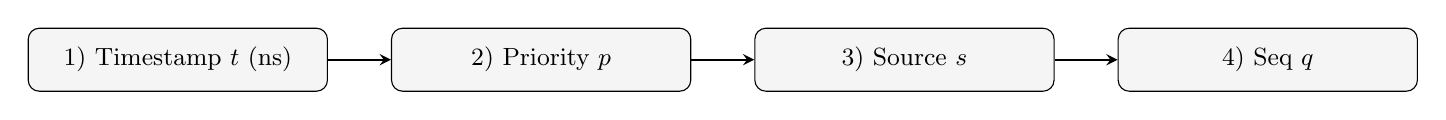
\begin{tikzpicture}[
    node distance=1.0cm,
    box/.style={rectangle, draw, rounded corners, align=center, font=\small, minimum height=0.8cm, minimum width=3.8cm, fill=boxgray},
    arrow/.style={->, >=stealth, thick}
]
    \node[box] (k1) {1) Timestamp $t$ (ns)};
    \node[box, right=0.8cm of k1] (k2) {2) Priority $p$};
    \node[box, right=0.8cm of k2] (k3) {3) Source $s$};
    \node[box, right=0.8cm of k3] (k4) {4) Seq $q$};
    \draw[arrow] (k1) -- (k2);
    \draw[arrow] (k2) -- (k3);
    \draw[arrow] (k3) -- (k4);
\end{tikzpicture}
\caption{EventQueue ordering key decomposition}
\end{figure}

% =============================================================================
\section{Market Data Ingestion and Normalization}
% =============================================================================

\subsection{MarketDataFeed Interface}
Market replay is abstracted behind a feed interface that supports incremental consumption, peeking, and reset for multi-run determinism.

\subsection{Normalization and Integrity Checks}
Historical data can be inconsistent (missing sequences, non-monotonic timestamps, invalid prices/sizes). The normalization layer converts raw formats into canonical events and tracks integrity statistics. A repair mode can resynchronize via last-known snapshots when deltas exhibit large sequence gaps.

\begin{figure}[h]
\centering
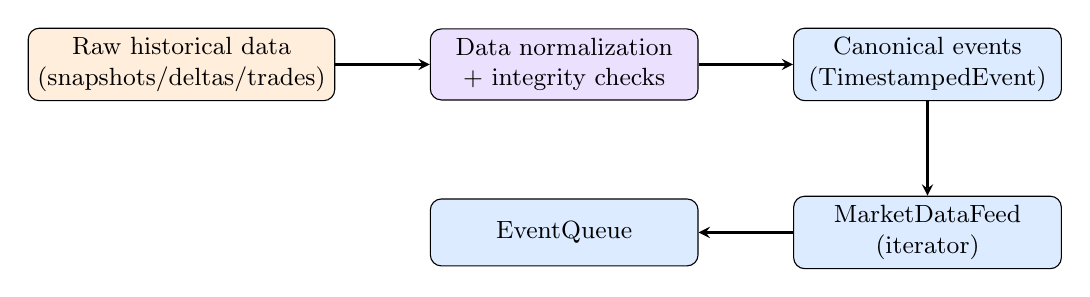
\begin{tikzpicture}[
    node distance=1.2cm,
    box/.style={rectangle, draw, rounded corners, align=center, minimum width=3.4cm, minimum height=0.85cm, font=\small},
    raw/.style={box, fill=boxorange},
    norm/.style={box, fill=boxpurple},
    canon/.style={box, fill=boxblue},
    arrow/.style={->, >=stealth, thick}
]
    \node[raw] (raw) {Raw historical data\\(snapshots/deltas/trades)};
    \node[norm, right=of raw] (dn) {Data normalization\\+ integrity checks};
    \node[canon, right=of dn] (ev) {Canonical events\\(TimestampedEvent)};
    \node[canon, below=of ev] (feed) {MarketDataFeed\\(iterator)};
    \node[canon, left=of feed] (q) {EventQueue};

    \draw[arrow] (raw) -- (dn);
    \draw[arrow] (dn) -- (ev);
    \draw[arrow] (ev) -- (feed);
    \draw[arrow] (feed) -- (q);
\end{tikzpicture}
\caption{Market data ingestion pipeline (conceptual)}
\end{figure}

\subsection{Book State Construction (Optional)}
While strategies may receive snapshot-like structures, a dedicated book manager can maintain consistent L2 state by applying snapshots and deltas, detect crossed-book conditions, and compute derived quantities (mid, spread, imbalance, depth, and simple impact estimates). This supports strategies that require stable multi-update book context.

% =============================================================================
\section{Strategy Surface: Production-Identical Interface}
% =============================================================================

\subsection{Callbacks and Responsibilities}
The strategy interface is callback-driven and event-synchronous: each callback receives a context containing (a) a mutable order interface and (b) the current simulation timestamp. The strategy is responsible for maintaining its own state machine (quoting, inventory control, throttling) using only these deterministic inputs.

\begin{table}[h]
\centering
\small
\begin{tabularx}{\textwidth}{@{}lX@{}}
\toprule
\textbf{Callback} & \textbf{When it fires and what it should do} \\
\midrule
\texttt{on\_start} & Initialize internal state, seed parameters, schedule recurring timers, optionally place initial orders. \\
\texttt{on\_book\_update} & Update microstructure state (best bid/ask, spread); decide quoting changes; submit/cancel/replace orders. \\
\texttt{on\_trade} & Update trade-based signals (momentum, toxicity); adjust quoting aggressiveness. \\
\texttt{on\_order\_ack} & Reconcile that an order is live; update outstanding order tracking and queue estimates. \\
\texttt{on\_order\_reject} & Backoff, reprice, or adjust rate to respect venue constraints; record failure statistics. \\
\texttt{on\_fill} & Update inventory and realized PnL; potentially hedge complement; adapt spread/size. \\
\texttt{on\_cancel\_ack} & Confirm removal of an order; resolve cancel-fill races when fills also occur. \\
\texttt{on\_timer} & Deterministic periodic actions (re-quote, decay signals, compute metrics, timeouts). \\
\texttt{on\_stop} & Final cleanup; export state snapshot if needed. \\
\bottomrule
\end{tabularx}
\caption{Strategy callbacks and expected responsibilities}
\end{table}

\subsection{OrderSender Contract}
Strategies interact with the venue through an abstract order sender. In backtests, this is backed by a simulator; in production, it would be backed by a live gateway.

\begin{figure}[h]
\centering
\begin{tikzpicture}[
    node distance=1.2cm,
    box/.style={rectangle, draw, rounded corners, align=center, minimum width=3.9cm, minimum height=0.9cm, font=\small},
    strat/.style={box, fill=boxblue},
    api/.style={box, fill=boxgray},
    impl/.style={box, fill=boxgreen},
    arrow/.style={->, >=stealth, thick},
    dashed/.style={->, >=stealth, thick, dashed}
]
    \node[strat] (s) {Strategy};
    \node[api, right=of s] (os) {OrderSender interface\\(send/cancel/query/timers)};
    \node[impl, right=of os] (sim) {SimulatedOrderSender};
    \node[impl, below=of sim] (live) {LiveOrderSender\\(future / external)};

    \draw[arrow] (s) -- (os);
    \draw[arrow] (os) -- (sim);
    \draw[dashed] (os) -- (live);
\end{tikzpicture}
\caption{Adapter boundary: strategy portability across backtest and live}
\end{figure}

% =============================================================================
\section{Simulated Execution Path}
% =============================================================================

\subsection{SimulatedOrderSender Responsibilities}
The simulated order sender implements the order interface and is responsible for:
\begin{itemize}[leftmargin=*,itemsep=2pt]
    \item sampling execution latencies (order send, venue processing, cancels),
    \item routing orders/cancels into the matching simulator at future simulated times,
    \item collecting the resulting order lifecycle events (acks, fills, rejects, cancels) and returning them to the orchestrator for deterministic scheduling,
    \item tracking open orders and lightweight position/PnL state for reporting.
\end{itemize}

\subsection{Latency Model: Components and Distributions}
Latency is modeled as a composition of independent distributions, each of which can be fixed or stochastic (uniform, normal, log-normal, exponential, gamma) with optional tail-spike mixtures.

\begin{table}[h]
\centering
\small
\begin{tabularx}{\textwidth}{@{}lX@{}}
\toprule
\textbf{Latency component} & \textbf{Interpretation} \\
\midrule
Market data & Exchange-to-strategy delay for book/trade visibility. \\
Decision & Strategy compute time between receiving data and issuing an action. \\
Order send & Strategy-to-gateway/network latency for new orders. \\
Venue processing & Gateway-to-matching-engine processing time. \\
Cancel processing & Cancel request latency. \\
Fill report & Exchange-to-strategy delay for fills/acks (if modeled separately). \\
\bottomrule
\end{tabularx}
\caption{Latency model components}
\end{table}

\begin{figure}[h]
\centering
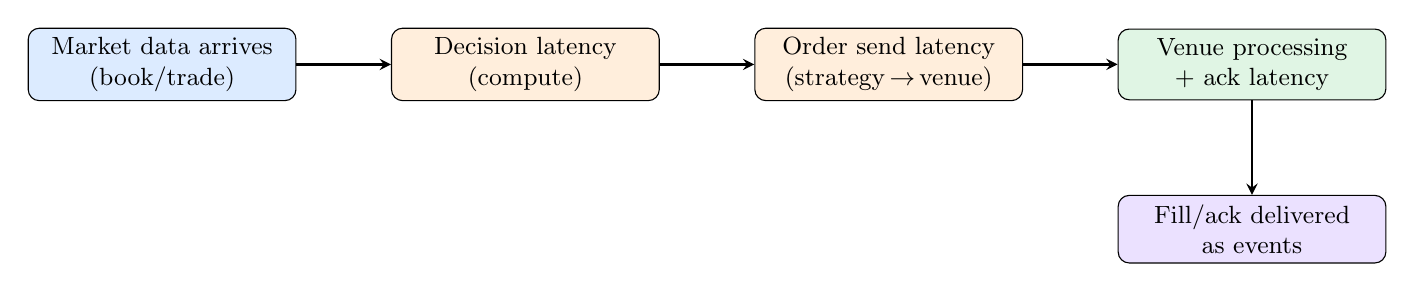
\begin{tikzpicture}[
    node distance=1.2cm,
    box/.style={rectangle, draw, rounded corners, align=center, minimum width=3.4cm, minimum height=0.85cm, font=\small},
    arrow/.style={->, >=stealth, thick}
]
    \node[box, fill=boxblue] (md) {Market data arrives\\(book/trade)};
    \node[box, fill=boxorange, right=of md] (dec) {Decision latency\\(compute)};
    \node[box, fill=boxorange, right=of dec] (send) {Order send latency\\(strategy\,$\to$\,venue)};
    \node[box, fill=boxgreen, right=of send] (venue) {Venue processing\\+ ack latency};
    \node[box, fill=boxpurple, below=of venue] (rep) {Fill/ack delivered\\as events};

    \draw[arrow] (md) -- (dec);
    \draw[arrow] (dec) -- (send);
    \draw[arrow] (send) -- (venue);
    \draw[arrow] (venue) -- (rep);
\end{tikzpicture}
\caption{Conceptual tick-to-trade latency pipeline}
\end{figure}

\subsection{Matching Simulator: LimitOrderBook and MatchingEngine}
Backtest V2 includes a full CLOB simulator with FIFO price level queues. Orders are discretized to integer ticks to preserve deterministic matching.

\paragraph{Tick discretization.} Binary markets trade in the $[0,1]$ probability range, typically with a fixed tick size (e.g., $0.01$). Prices are mapped to integer ticks and clamped to a valid range.

\begin{table}[h]
\centering
\small
\begin{tabularx}{\textwidth}{@{}lX@{}}
\toprule
\textbf{Matching config field} & \textbf{Effect on simulation} \\
\midrule
Tick size & Controls price discretization and level indexing. \\
Maker/taker fees & Applies per-fill fees (maker can be negative for rebates). \\
Self-trade prevention & Prevents a strategy from matching against itself; multiple STP policies exist (cancel newest/oldest/both). \\
Min/max order size & Order validity constraints. \\
Ack latency & Additional time added before order acknowledgments and fill events are emitted. \\
\bottomrule
\end{tabularx}
\caption{Matching configuration: high-level semantics}
\end{table}

\begin{figure}[h]
\centering
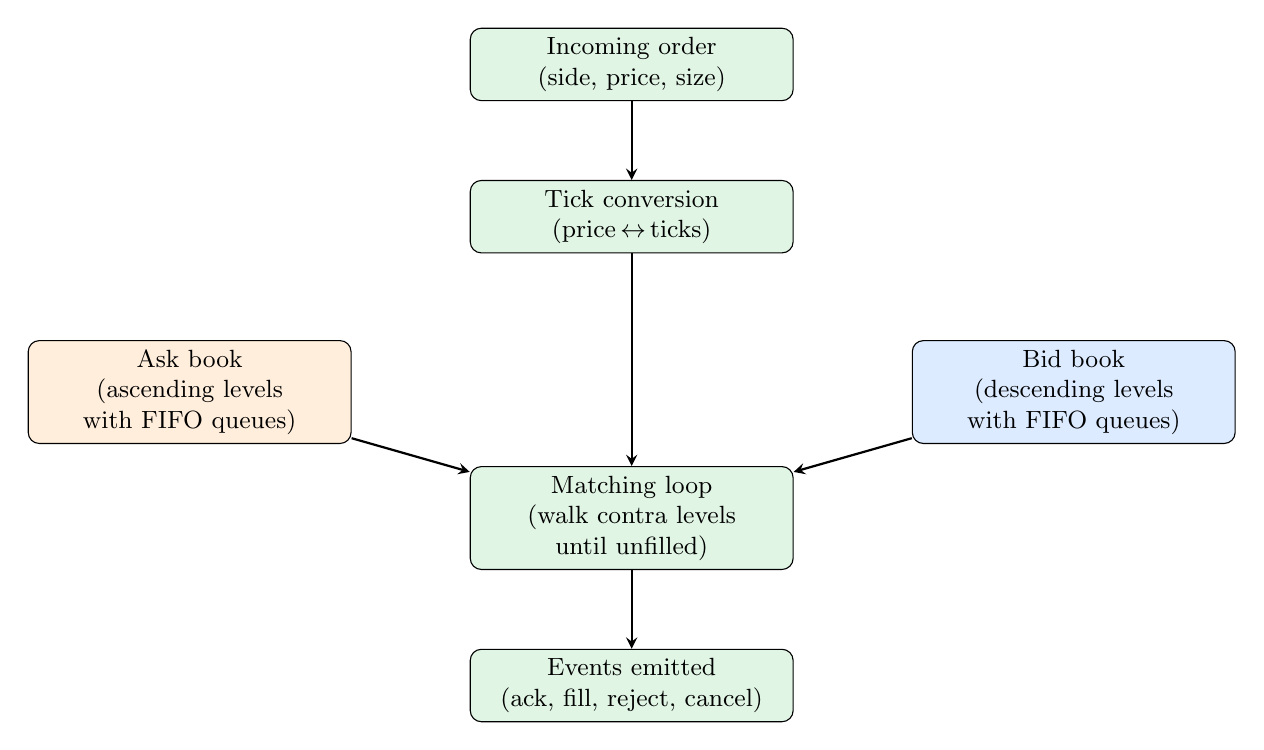
\begin{tikzpicture}[
    node distance=1.0cm,
    box/.style={rectangle, draw, rounded corners, align=center, minimum width=4.1cm, minimum height=0.9cm, font=\small},
    bid/.style={box, fill=boxblue},
    ask/.style={box, fill=boxorange},
    core/.style={box, fill=boxgreen},
    arrow/.style={->, >=stealth, thick}
]
    \node[core] (in) {Incoming order\\(side, price, size)};
    \node[core, below=of in] (ticks) {Tick conversion\\(price\,$\leftrightarrow$\,ticks)};
    \node[ask, below left=1.1cm and 1.5cm of ticks] (asks) {Ask book\\(ascending levels\\with FIFO queues)};
    \node[bid, below right=1.1cm and 1.5cm of ticks] (bids) {Bid book\\(descending levels\\with FIFO queues)};
    \node[core, below=2.7cm of ticks] (match) {Matching loop\\(walk contra levels\\until unfilled)};
    \node[core, below=of match] (out) {Events emitted\\(ack, fill, reject, cancel)};

    \draw[arrow] (in) -- (ticks);
    \draw[arrow] (ticks) -- (match);
    \draw[arrow] (asks) -- (match);
    \draw[arrow] (bids) -- (match);
    \draw[arrow] (match) -- (out);
\end{tikzpicture}
\caption{Matching simulator structure (single-token view)}
\end{figure}

\subsection{Order Types and Time-in-Force Semantics}
Backtest V2 models common order constraints:
\begin{itemize}[leftmargin=*,itemsep=2pt]
    \item \textbf{Post-only:} order is rejected if it would immediately cross the spread.
    \item \textbf{GTC/GTT:} unfilled remainder becomes resting liquidity.
    \item \textbf{IOC/FOK:} any unfilled remainder is cancelled immediately (IOC) or the order is rejected/cancelled if it cannot fully execute (FOK).
\end{itemize}

\subsection{Cancel-Fill Races and Queue Modeling (Optional)}
In real markets, cancels compete with fills at the venue. Backtest V2 provides a queue position model that tracks FIFO position at each price level and can report cancel-fill race outcomes (cancel wins, fill wins, partial). This enables more realistic evaluation of passive strategies where queue position materially impacts fill probability.

% =============================================================================
\section{OMS (Order Management System): State Machine + Venue Constraints}
% =============================================================================

\subsection{Role in Architecture}
The OMS provides a realistic order lifecycle state machine, pre-trade validation against venue constraints, rate limiting, and defenses against out-of-order message delivery. In richer orchestrations, the OMS sits between strategy intent and the matching/venue adapter.

\subsection{Order State Machine}
\begin{figure}[h]
\centering
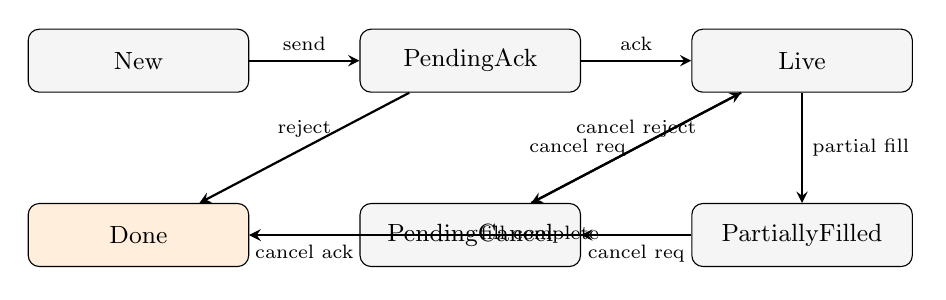
\begin{tikzpicture}[
    node distance=1.4cm,
    state/.style={rectangle, draw, rounded corners, align=center, minimum width=2.8cm, minimum height=0.8cm, font=\small, fill=boxgray},
    terminal/.style={state, fill=boxorange},
    arrow/.style={->, >=stealth, thick}
]
    \node[state] (new) {New};
    \node[state, right=of new] (pendack) {PendingAck};
    \node[state, right=of pendack] (live) {Live};
    \node[state, below=of live] (partial) {PartiallyFilled};
    \node[state, left=of partial] (pendcxl) {PendingCancel};
    \node[terminal, left=of pendcxl] (done) {Done};

    \draw[arrow] (new) -- node[font=\scriptsize, above]{send} (pendack);
    \draw[arrow] (pendack) -- node[font=\scriptsize, above]{ack} (live);
    \draw[arrow] (pendack) -- node[font=\scriptsize, above]{reject} (done);
    \draw[arrow] (live) -- node[font=\scriptsize, right]{partial fill} (partial);
    \draw[arrow] (partial) -- node[font=\scriptsize, right]{fill complete} (done);
    \draw[arrow] (live) -- node[font=\scriptsize, left]{cancel req} (pendcxl);
    \draw[arrow] (partial) -- node[font=\scriptsize, below]{cancel req} (pendcxl);
    \draw[arrow] (pendcxl) -- node[font=\scriptsize, below]{cancel ack} (done);
    \draw[arrow] (pendcxl) -- node[font=\scriptsize, above]{cancel reject} (live);
\end{tikzpicture}
\caption{OMS order state machine (high-level)}
\end{figure}

\subsection{Venue Constraints and Rate Limiting}
The OMS validates orders against constraints such as min/max size, tick conformance, allowed order types and time-in-force, and maximum open orders. A sliding-window rate limiter enforces order and cancel throughput limits.

\begin{table}[h]
\centering
\small
\begin{tabularx}{\textwidth}{@{}lX@{}}
\toprule
\textbf{Constraint class} & \textbf{Examples} \\
\midrule
Order validity & price range, tick-size alignment, size bounds \\
Venue feature flags & post-only allowed, reduce-only allowed, allowed order types \\
Capacity limits & max open orders per token, max total open orders \\
Rate limits & max orders per second, max cancels per second \\
Market status gating & open vs halted vs resolving vs closed \\
\bottomrule
\end{tabularx}
\caption{OMS constraint categories}
\end{table}

% =============================================================================
\section{Risk and Portfolio Accounting}
% =============================================================================

\subsection{Portfolio: Positions, PnL, and Settlement}
The portfolio subsystem models cash, outcome-token positions, fees, realized/unrealized PnL, equity curves, and settlement for binary markets. A market-level position bundles YES and NO outcomes to enable complement coupling and worst-case exposure computation.

\begin{figure}[h]
\centering
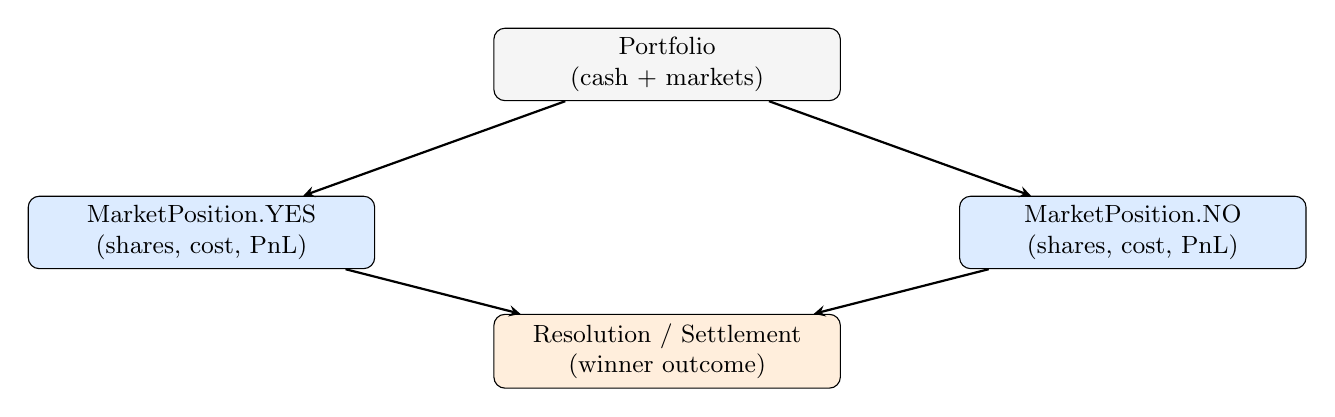
\begin{tikzpicture}[
    node distance=1.2cm,
    box/.style={rectangle, draw, rounded corners, align=center, minimum width=4.4cm, minimum height=0.85cm, font=\small},
    arrow/.style={->, >=stealth, thick}
]
    \node[box, fill=boxgray] (pf) {Portfolio\\(cash + markets)};
    \node[box, fill=boxblue, below left=1.2cm and 1.5cm of pf] (yes) {MarketPosition.YES\\(shares, cost, PnL)};
    \node[box, fill=boxblue, below right=1.2cm and 1.5cm of pf] (no) {MarketPosition.NO\\(shares, cost, PnL)};
    \node[box, fill=boxorange, below=2.7cm of pf] (settle) {Resolution / Settlement\\(winner outcome)};

    \draw[arrow] (pf) -- (yes);
    \draw[arrow] (pf) -- (no);
    \draw[arrow] (yes) -- (settle);
    \draw[arrow] (no) -- (settle);
\end{tikzpicture}
\caption{Portfolio model: market-level YES/NO coupling and settlement}
\end{figure}

\subsection{RiskManager: Pre-Trade Checks and Kelly Sizing}
Risk management combines two layers:
\begin{enumerate}[leftmargin=*,itemsep=2pt]
    \item \textbf{Sizing (Kelly):} converts an estimated edge into a target position fraction subject to caps and minimum edge thresholds.
    \item \textbf{Hard limits:} blocks or reduces orders based on exposure, per-market concentration, outstanding order counts, cash buffers, drawdown stops, and daily limits.
\end{enumerate}

\begin{table}[h]
\centering
\small
\begin{tabularx}{\textwidth}{@{}lX@{}}
\toprule
\textbf{Risk limit} & \textbf{High-level meaning} \\
\midrule
Gross exposure multiple & Bounds total deployed exposure as a multiple of equity. \\
Max per-market position & Prevents concentration in a single market/outcome. \\
Max order size / notional & Guards against fat-finger or pathological sizing. \\
Outstanding order caps & Limits operational complexity and queue spam. \\
Drawdown stop + cooldown & Halts trading after a large loss and enforces a backoff window. \\
Min cash balance & Maintains liquidity buffer for safety and fees. \\
Daily loss / trade limits & Enforces ``circuit breakers'' and prevents runaway activity. \\
\bottomrule
\end{tabularx}
\caption{RiskManager checks (summary)}
\end{table}

\begin{figure}[h]
\centering
\begin{tikzpicture}[
    node distance=1.2cm,
    box/.style={rectangle, draw, rounded corners, align=center, minimum width=3.6cm, minimum height=0.85cm, font=\small},
    arrow/.style={->, >=stealth, thick},
    dashed/.style={->, >=stealth, thick, dashed}
]
    \node[box, fill=boxblue] (sig) {Strategy intent\\(side, price, size)};
    \node[box, fill=boxpurple, right=of sig] (kelly) {Kelly sizing\\(edge\,$\to$\,target size)};
    \node[box, fill=boxorange, right=of kelly] (risk) {Risk checks\\(block/reduce)};
    \node[box, fill=boxgray, right=of risk] (route) {Route to OMS\\/ adapter};

    \draw[arrow] (sig) -- (kelly);
    \draw[arrow] (kelly) -- (risk);
    \draw[arrow] (risk) -- (route);
    \draw[dashed] (risk) to[bend left=30] node[font=\scriptsize, above]{log blocked} (sig);
\end{tikzpicture}
\caption{Conceptual pre-trade decision pipeline (sizing + risk gating)}
\end{figure}

% =============================================================================
\section{Metrics and Backtest Reporting}
% =============================================================================

\subsection{MetricsCollector Overview}
Backtest V2 includes a comprehensive metrics system designed for microstructure evaluation as well as portfolio-level performance. Metrics are organized into domains:
\begin{itemize}[leftmargin=*,itemsep=2pt]
    \item \textbf{Latency:} distributions for order-to-ack, ack-to-fill, cancel-to-ack, and strategy compute proxies.
    \item \textbf{Fills:} fill rates, cancel rates, reject rates, maker/taker mix, fees, and time-in-queue percentiles.
    \item \textbf{Slippage:} distribution of execution price vs mid (at order or fill time).
    \item \textbf{Adverse selection:} PnL at multiple horizons after fill (toxicity proxy).
    \item \textbf{Tail risk:} drawdowns and rolling worst PnL windows (Calmar-style summaries).
    \item \textbf{Per-market breakdown:} fill counts, volume, fees, realized/unrealized PnL, maker ratios, average slippage.
\end{itemize}

\begin{table}[h]
\centering
\small
\begin{tabularx}{\textwidth}{@{}lX@{}}
\toprule
\textbf{Metric family} & \textbf{What it answers} \\
\midrule
Latency percentiles & ``How fast is the strategy + execution loop, and how heavy are tails?'' \\
Fill and cancel rates & ``Do quotes actually trade, or do we churn and miss fills?'' \\
Slippage & ``Are we paying spread / moving the market?'' \\
Adverse selection & ``Are fills informed against us at +100ms/+1s/+1m horizons?'' \\
Tail risk & ``What is the worst short-window PnL and maximum drawdown?'' \\
Per-market attribution & ``Which markets contribute returns and risk?'' \\
\bottomrule
\end{tabularx}
\caption{Metrics: interpretability guide}
\end{table}

\begin{figure}[h]
\centering
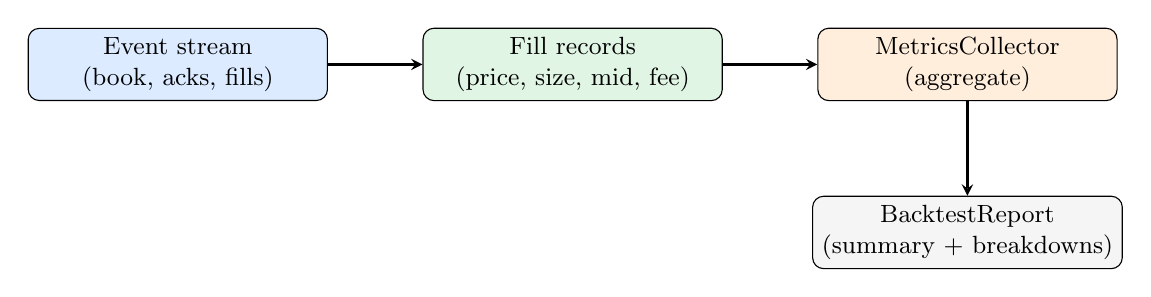
\begin{tikzpicture}[
    node distance=1.2cm,
    box/.style={rectangle, draw, rounded corners, align=center, minimum width=3.8cm, minimum height=0.85cm, font=\small},
    arrow/.style={->, >=stealth, thick}
]
    \node[box, fill=boxblue] (events) {Event stream\\(book, acks, fills)};
    \node[box, fill=boxgreen, right=of events] (fills) {Fill records\\(price, size, mid, fee)};
    \node[box, fill=boxorange, right=of fills] (metrics) {MetricsCollector\\(aggregate)};
    \node[box, fill=boxgray, below=of metrics] (report) {BacktestReport\\(summary + breakdowns)};

    \draw[arrow] (events) -- (fills);
    \draw[arrow] (fills) -- (metrics);
    \draw[arrow] (metrics) -- (report);
\end{tikzpicture}
\caption{Metrics data flow (conceptual)}
\end{figure}

% =============================================================================
\section{Validation and Reproducibility}
% =============================================================================

\subsection{Deterministic Seeding}
Backtest V2 provides a deterministic seed structure that derives sub-seeds for different stochastic subsystems (latency sampling, fill probability, queue modeling). This reduces accidental coupling between randomness sources and improves reproducibility.

\subsection{State Fingerprinting and Checkpoints}
To detect divergences across runs, the validator can record periodic checkpoints containing a state fingerprint (timestamp, event counts, cash, and hashes of positions and book state). Two runs can be compared by checkpoint sequence to localize the first divergence.

\subsection{Invariant Checking}
An invariant checker can validate order book properties (e.g., not crossed, non-negative sizes, valid price ranges) and detect overfills or references to unknown orders.

\begin{table}[h]
\centering
\small
\begin{tabularx}{\textwidth}{@{}lX@{}}
\toprule
\textbf{Invariant category} & \textbf{Example violation} \\
\midrule
Book topology & best bid $\ge$ best ask (crossed book) \\
Numeric validity & negative size at a level; price outside $[0,1]$ \\
Order lifecycle coherence & fills exceeding available quantity; unknown order references \\
Custom invariants & user-defined checks for strategy/accounting consistency \\
\bottomrule
\end{tabularx}
\caption{Invariant checking categories}
\end{table}

\subsection{Trace Mode}
Trace mode records an ordered event log including market data, strategy actions, order lifecycle transitions, fills, and book/portfolio snapshots. This supports forensic debugging when a strategy behaves unexpectedly.

\begin{figure}[h]
\centering
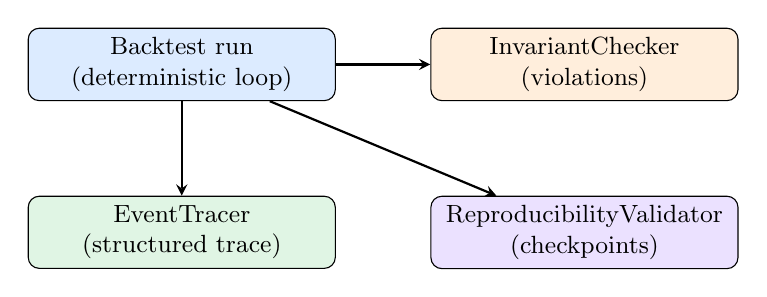
\begin{tikzpicture}[
    node distance=1.2cm,
    box/.style={rectangle, draw, rounded corners, align=center, minimum width=3.9cm, minimum height=0.85cm, font=\small},
    arrow/.style={->, >=stealth, thick}
]
    \node[box, fill=boxblue] (run) {Backtest run\\(deterministic loop)};
    \node[box, fill=boxorange, right=of run] (inv) {InvariantChecker\\(violations)};
    \node[box, fill=boxpurple, below=of inv] (fp) {ReproducibilityValidator\\(checkpoints)};
    \node[box, fill=boxgreen, below=of run] (trace) {EventTracer\\(structured trace)};

    \draw[arrow] (run) -- (inv);
    \draw[arrow] (run) -- (fp);
    \draw[arrow] (run) -- (trace);
\end{tikzpicture}
\caption{Validation harness components}
\end{figure}

% =============================================================================
\section{Performance and Scaling Toolkit}
% =============================================================================

\subsection{Zero-Allocation Hot Path Tools}
To reduce allocation pressure in high-event-rate simulations, Backtest V2 includes pre-allocated pools:
\begin{itemize}[leftmargin=*,itemsep=2pt]
    \item \textbf{EventPool:} reusable buffer for timestamped events.
    \item \textbf{LevelPool:} reusable buffers for bid/ask level vectors.
    \item \textbf{StringArena:} bump allocator for short-lived strings.
\end{itemize}

\subsection{Per-Market Isolation and Parallelization}
The performance module introduces a per-market \emph{isolated state} concept (book, config, seed, and pools) that can be processed independently. Events can be partitioned by market and processed in parallel while preserving determinism within each market.

\begin{figure}[h]
\centering
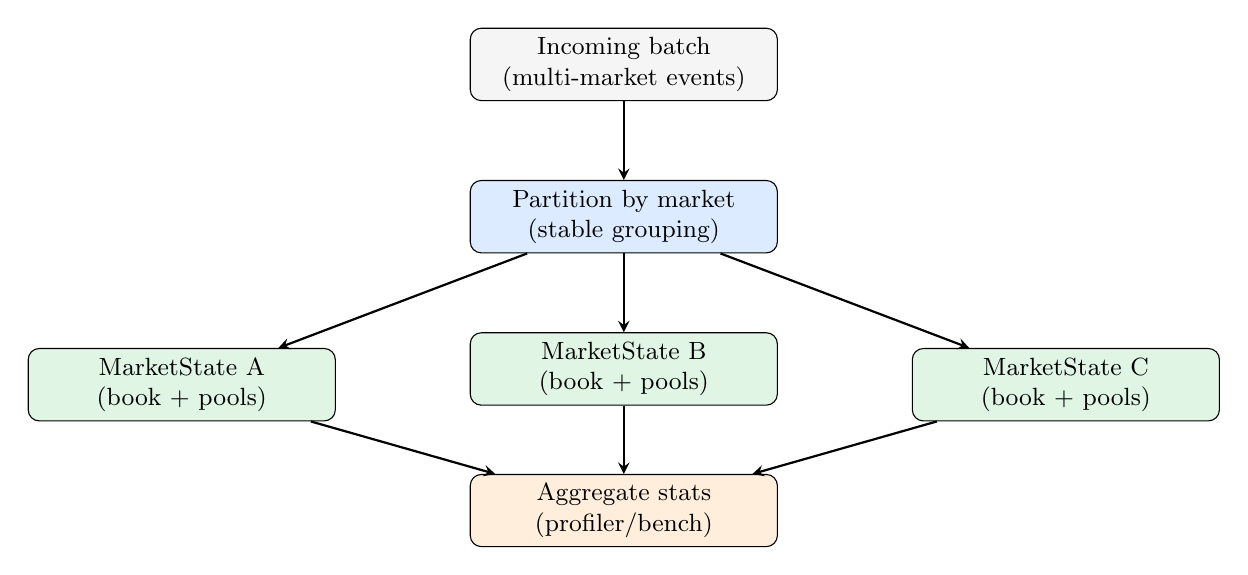
\begin{tikzpicture}[
    node distance=1.0cm,
    box/.style={rectangle, draw, rounded corners, align=center, minimum width=3.9cm, minimum height=0.8cm, font=\small},
    arrow/.style={->, >=stealth, thick}
]
    \node[box, fill=boxgray] (batch) {Incoming batch\\(multi-market events)};
    \node[box, fill=boxblue, below=of batch] (partition) {Partition by market\\(stable grouping)};
    \node[box, fill=boxgreen, below left=1.2cm and 1.7cm of partition] (m1) {MarketState A\\(book + pools)};
    \node[box, fill=boxgreen, below=of partition] (m2) {MarketState B\\(book + pools)};
    \node[box, fill=boxgreen, below right=1.2cm and 1.7cm of partition] (m3) {MarketState C\\(book + pools)};
    \node[box, fill=boxorange, below=2.8cm of partition] (agg) {Aggregate stats\\(profiler/bench)};

    \draw[arrow] (batch) -- (partition);
    \draw[arrow] (partition) -- (m1);
    \draw[arrow] (partition) -- (m2);
    \draw[arrow] (partition) -- (m3);
    \draw[arrow] (m1) -- (agg);
    \draw[arrow] (m2) -- (agg);
    \draw[arrow] (m3) -- (agg);
\end{tikzpicture}
\caption{Parallel processing concept: per-market isolated state}
\end{figure}

\subsection{Profiling and Benchmarks}
The profiler records per-stage durations (event parsing, book updates, matching, fill processing, strategy callback, risk checks, portfolio updates, metrics) and can emit a terminal-oriented summary. Benchmark runners can stress throughput and memory efficiency under controlled synthetic loads.

% =============================================================================
\section{Configuration Surfaces (Summary Tables)}
% =============================================================================

\subsection{BacktestConfig}
\begin{table}[h]
\centering
\small
\begin{tabularx}{\textwidth}{@{}lX@{}}
\toprule
\textbf{Field} & \textbf{Meaning} \\
\midrule
Matching config & Tick size, fees, STP policy, ack latency, size limits. \\
Latency config & Distributions for each latency stage; seeded sampling. \\
Strategy params & Read-only parameter bag passed to strategy context. \\
Trader id & Identifier used for self-trade prevention and attribution. \\
Seed & Global determinism seed (used for RNG seeding). \\
Max events & Optional cap to bound simulation length. \\
Verbose & Optional diagnostic verbosity control. \\
\bottomrule
\end{tabularx}
\caption{Backtest configuration fields (conceptual)}
\end{table}

\subsection{MatchingConfig}
\begin{table}[h]
\centering
\small
\begin{tabular}{@{}ll@{}}
\toprule
\textbf{Parameter} & \textbf{Example intent} \\
\midrule
Tick size & $0.01$ for cent ticks in $[0,1]$ prices \\
Taker fee rate & e.g., $10$ bps \\
Maker fee rate & $0$ or negative for rebate \\
STP enabled + mode & cancel newest/oldest/both \\
Min/max order size & prevent invalid orders \\
Ack latency & event emission delay for acks/fills/cancels \\
\bottomrule
\end{tabular}
\caption{Matching configuration: key knobs}
\end{table}

\subsection{RiskLimits (Representative)}
\begin{table}[h]
\centering
\small
\begin{tabularx}{\textwidth}{@{}lX@{}}
\toprule
\textbf{Limit} & \textbf{Purpose} \\
\midrule
Max gross exposure multiple & Prevents leverage blow-ups across many markets. \\
Max per-market exposure & Prevents concentration in a single binary outcome. \\
Min cash buffer & Preserves ability to exit and pay fees. \\
Daily loss/trade caps & Circuit breakers for pathological regimes. \\
Cooldown interval & Enforced pause after a stop condition. \\
\bottomrule
\end{tabularx}
\caption{Risk limit configuration (summary)}
\end{table}

% =============================================================================
\section{Practical Composition Patterns}
% =============================================================================

\subsection{Minimal Backtest Composition}
The smallest viable configuration composes:
\begin{enumerate}[leftmargin=*,itemsep=2pt]
    \item a feed producing timestamped market events,
    \item an orchestrator with a deterministic event queue,
    \item a strategy implementing the callback interface,
    \item a simulated order sender backed by a matching engine.
\end{enumerate}

\subsection{Richer ``Research-Grade'' Composition}
For microstructure and risk realism, a common extension is:
\begin{itemize}[leftmargin=*,itemsep=2pt]
    \item maintain full L2 state via book manager (instead of snapshot-only views),
    \item integrate OMS to enforce rate limits and handle out-of-order lifecycle events,
    \item incorporate queue position modeling to estimate passive fill probabilities and cancel-fill races,
    \item run ValidationHarness checkpoints to guarantee deterministic replay,
    \item record full MetricsCollector output for post-run analysis.
\end{itemize}

\subsection{Production Parity Principle}
Backtest V2 is designed around a stable boundary: the strategy sees only a deterministic time source, market events, and the order interface. Production parity is achieved by swapping the order sender implementation, not by rewriting strategy logic.

% =============================================================================
\section{Appendix: Diagram Legend and Reading Guide}
% =============================================================================

\begin{table}[h]
\centering
\small
\begin{tabular}{@{}ll@{}}
\toprule
\textbf{Visual element} & \textbf{Meaning} \\
\midrule
Blue boxes & Core orchestration and strategy surfaces \\
Green boxes & Simulation internals (matching, adapter) \\
Orange boxes & Constraints / realism / risk / latency emphasis \\
Purple boxes & Validation and reproducibility tooling \\
Gray boxes & Data containers / generic glue components \\
Dashed arrows & Optional or compositional integration points \\
\bottomrule
\end{tabular}
\caption{Legend for figures in this document}
\end{table}

\end{document}
